
%\documentclass[mathserif]{beamer}
\documentclass[handout]{beamer}
%\usetheme{Goettingen}
%\usetheme{Warsaw}
\usetheme{Singapore}



%\usetheme{Frankfurt}
%\usetheme{Copenhagen}
%\usetheme{Szeged}
%\usetheme{Montpellier}
%\usetheme{CambridgeUS}
%\usecolortheme{}
%\setbeamercovered{transparent}
\usepackage[english, activeacute]{babel}
\usepackage[utf8]{inputenc}
\usepackage{amsmath, amssymb}
\usepackage{dsfont}
\usepackage{graphics}
\usepackage{cases}
\usepackage{graphicx}
\usepackage{pgf}
\usepackage{epsfig}
\usepackage{amssymb}
\usepackage{multirow}	
\usepackage{amstext}
\usepackage[ruled,vlined,lined]{algorithm2e}
\usepackage{amsmath}
\usepackage{epic}
\usepackage{epsfig}
\usepackage{fontenc}
\usepackage{framed,color}
\usepackage{palatino, url, multicol}
%\algsetup{indent=2em}
\newcommand{\factorial}{\ensuremath{\mbox{\sc Factorial}}}
\newcommand{\BIGOP}[1]{\mathop{\mathchoice%
{\raise-0.22em\hbox{\huge $#1$}}%
{\raise-0.05em\hbox{\Large $#1$}}{\hbox{\large $#1$}}{#1}}}
\newcommand{\bigtimes}{\BIGOP{\times}}
\vspace{-0.5cm}
\title{Natural Language Processing \\ Large Language Models Usage and Evaluation Patterns}
\vspace{-0.5cm}
\author[Felipe Bravo Márquez]{\footnotesize
%\author{\footnotesize  
 \textcolor[rgb]{0.00,0.00,1.00}{Felipe Bravo-Marquez}} 
  
 

\date{\today}

\begin{document}
\begin{frame}
\titlepage


\end{frame}



\section{Introduction}
\begin{frame}{Introduction}
\begin{scriptsize}
\begin{itemize}
\item Since the inception of Large Language Models, various patterns of use and evaluation of this technology have emerged.
\item In this talk, we will try to organize these patterns and give a general overview of them.
\end{itemize}

 \begin{figure}[h]
        	
\includegraphics[scale = 0.2]{pics/Large-Language-Models.jpg}
        \end{figure}
Source: \url{https://www.masayume.it/img/masayume/Large-Language-Models.jpg}
\end{scriptsize}
\end{frame}



\begin{frame}{Recap: What is an LLM}
\begin{scriptsize}
\begin{itemize}
\item  An autoregressive language model trained with a Transformer neural network on a large corpus (hundreds of bullions of tokens) and a large parameter space (billions) to predict the next word.
\item It is usually later aligned to work as a user assistant using techniques such as Reinforcement Learning From Human Feedback  \cite{ouyang2022training} or supervised fine-tuning.
\item Some are private (access via API or web browser): Google Bard, ChatGPT, etc.
\item Others are open (model's weights can be downloaded): Llama, LLama2, Falcon, etc.
\item The most remarkable feature of these models is their few-shot, one-shot, zero-shot learning capabilities.
\item This means that they can learn new tasks without large amounts of human-annotated data.
\end{itemize}
\end{scriptsize}
\end{frame}

\begin{frame}{Zero-shot, One-shot, and Few-shot Learning}


 \begin{figure}[h]
        	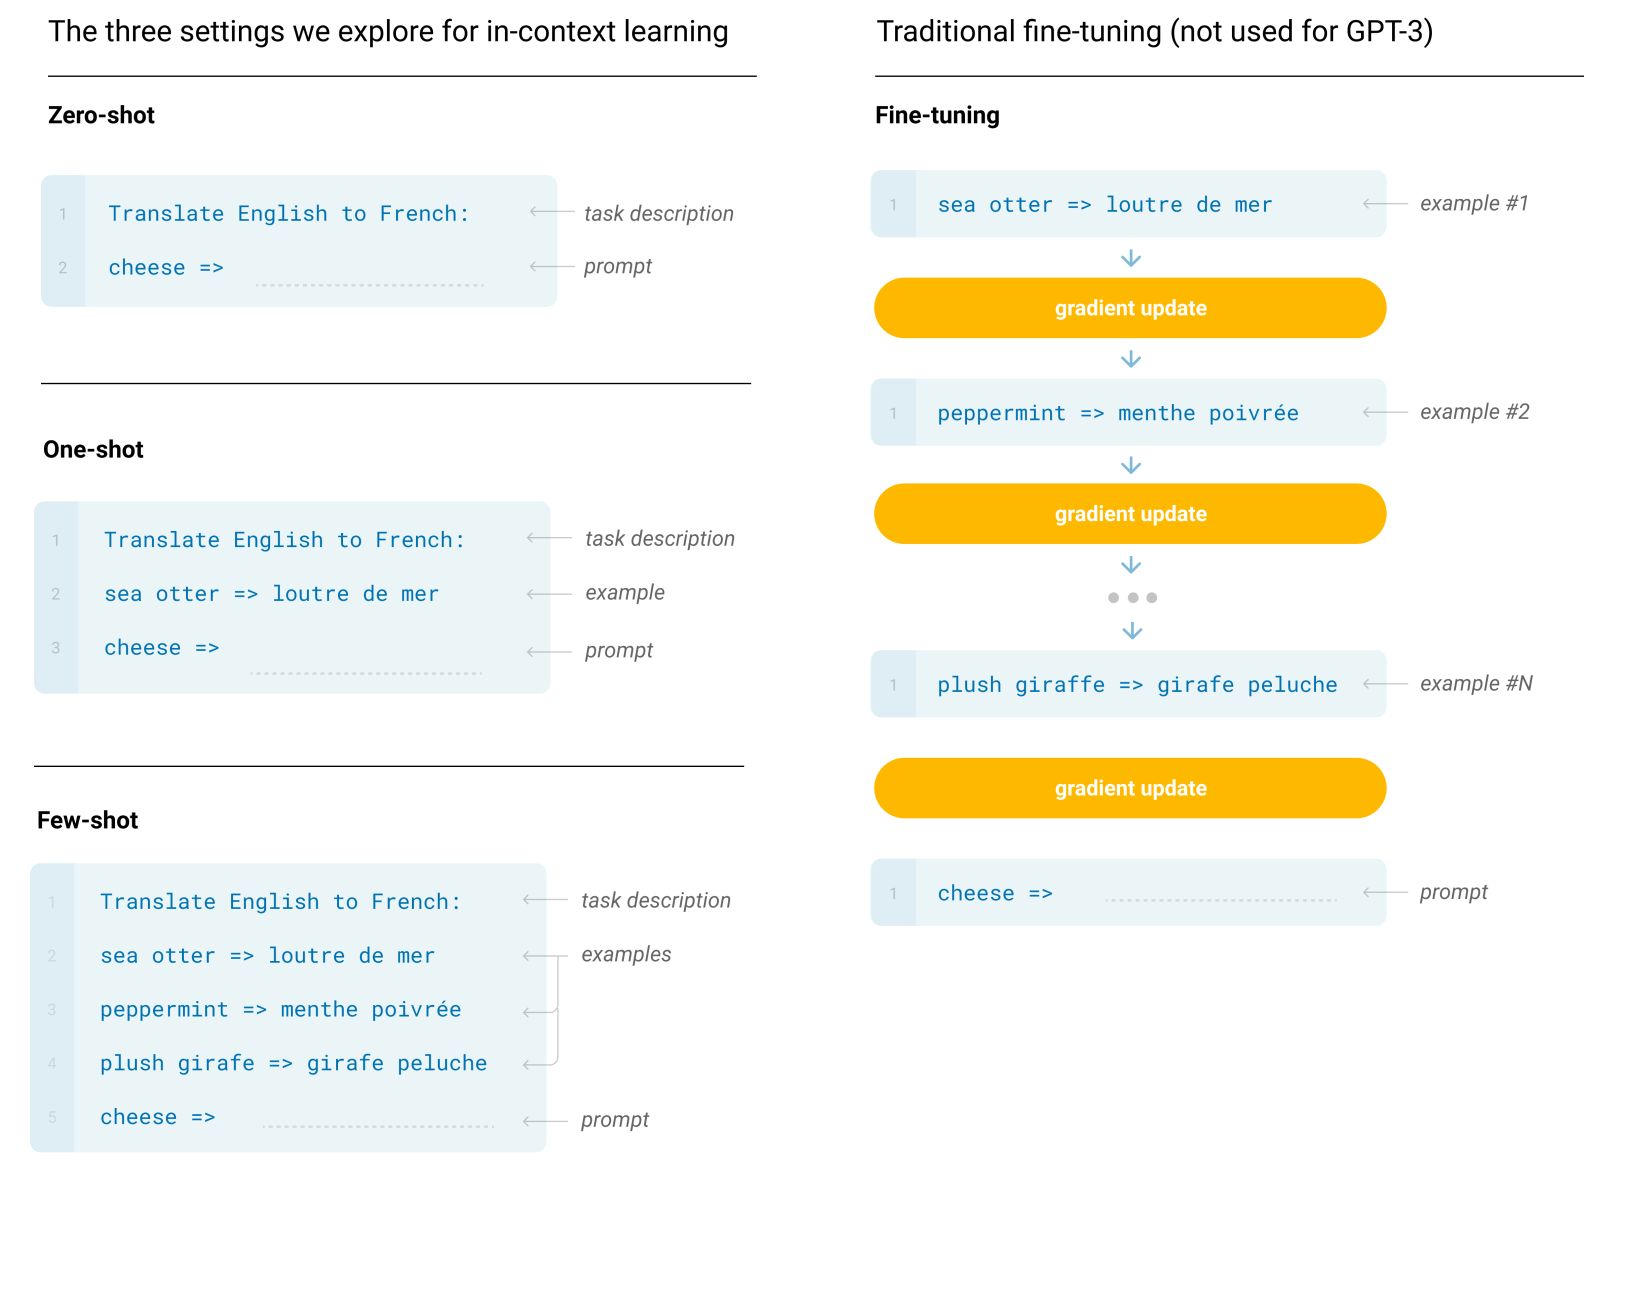
\includegraphics[scale = 0.18]{pics/zeroonefew.png}
        \end{figure}  



\end{frame}


\begin{frame}{Talk Overview}
\begin{scriptsize}
\begin{itemize}
 \item Despite the recency of this technology, its adoption has been tremendous in many areas. 
 \item Below, we propose a simple categorization of the ways in which LLMs are used and evaluated.
  \item These patterns will serve as the narrative backbone of this presentation.
\end{itemize}



\begin{columns}[t]
\column{0.5\textwidth}
\begin{block}{Usage Patterns}
\begin{enumerate}
\item Fixed-knowledge Assistant
\item Knowledge-augmented Assistant
\item LLM-based Applications 
\end{enumerate}
\end{block}

\column{0.5\textwidth}
\begin{block}{Evaluation Patterns}
\begin{itemize}
\item MTBench
\item LLM Arena
\end{itemize}
\end{block}

\end{columns}

\end{scriptsize}
\end{frame}









% \url{https://ai.meta.com/llama/get-started/?trk=feed_main-feed-card_reshare_feed-article-content}.

\section{Fixed-Knowledge Assistant}

\begin{frame}[fragile]{Usage Pattern 1: Fixed-Knowledge Assistant}
\begin{scriptsize}
\begin{itemize}
\item In this pattern a user interacts with the LLM proving prompts as input and receiving a text as answer.
\item The knowledge the LLM has access is limited to the corpus on which it was trained and the context given in the prompt.
\end{itemize}
\end{scriptsize}
\end{frame}



\begin{frame}[fragile]{Prompting}
\begin{scriptsize}
\begin{itemize}
\item Prompt Engineering : https://twitter.com/IntuitMachine/status/1727079666001870877
\item Roles
\item JSON outputs
\begin{verbatim}
   {"role": "system", "content": "You are a helpful assistant designed to output JSON."},
    {"role": "user", "content": "Who won the world series in 2020?"}
\end{verbatim}


\item Chain of thought Prompting
\end{itemize}
\end{scriptsize}
\end{frame}


\section{Knowledge-augmented Assistant}

\begin{frame}{Knowledge-augmented Assistant}
\begin{scriptsize}
\begin{itemize}
\item Idea incorporate domain-scpefific knowledge not included during training.
\item There two main patterns to achieve this:
\begin{enumerate}\scriptsize
 \item Retrieval-Augmented Generation (Vector Databases)
 \item Instruction Fine-Tuning
\end{enumerate}
\end{itemize}

    Setting the style, tone, format, or other qualitative aspects
    Improving reliability at producing a desired output
    Correcting failures to follow complex prompts
    Handling many edge cases in specific ways
    Performing a new skill or task that’s hard to articulate in a prompt

\end{scriptsize}
% https://platform.openai.com/docs/guides/fine-tuning/common-use-cases
\end{frame}


\begin{frame}{Retrieval-Augmented Generation}
\begin{scriptsize}
\begin{itemize}
\item Rely on a Vector Database embed queries, retrieve relevant documents, append them into the prompt
\cite{lewis2021retrievalaugmented}.
\item Many ideas of Informatrion Retrieval are employed here.

\item \url{https://www.infoworld.com/article/3709912/vector-databases-in-llms-and-search.html}
\item \url{https://learn.deeplearning.ai/vector-databases-embeddings-applications/lesson/1/introduction}
\item \url{https://stackoverflow.blog/2023/10/09/from-prototype-to-production-vector-databases-in-generative-ai-applications/}
\end{itemize}
\end{scriptsize}

    \begin{figure}[h]
        	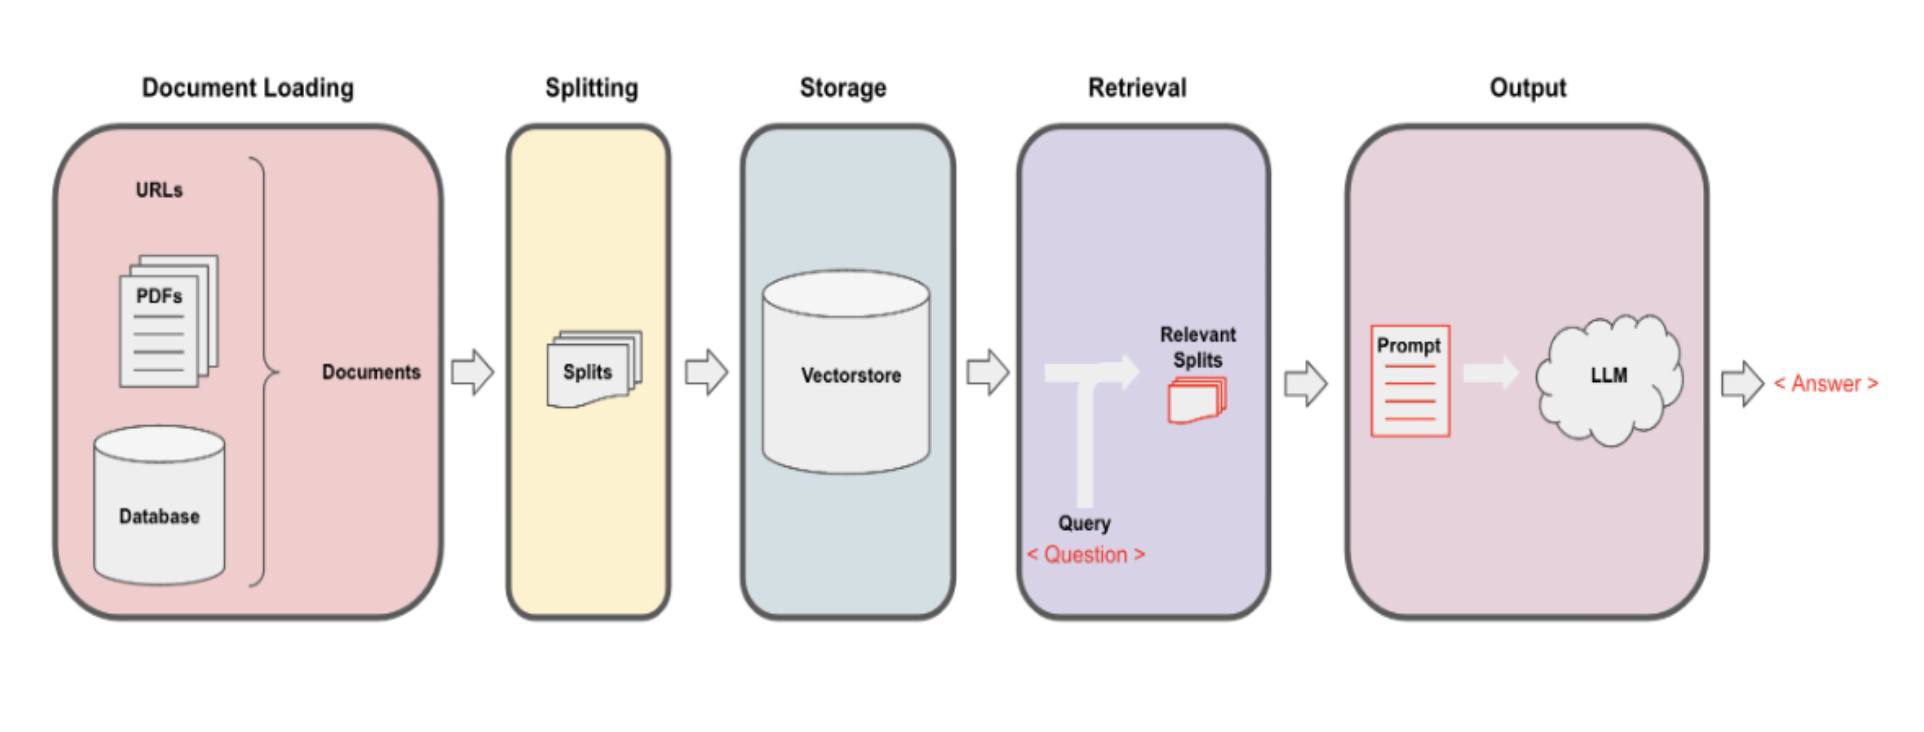
\includegraphics[scale = 0.2]{pics/vectordatabase.png}
        \end{figure}  


\end{frame}



\begin{frame}{Instruction Fine-Tuning}
\begin{scriptsize}
\begin{itemize}
\item Idea: instead of training the LM with raw text with next token prediction, train it with pairs of prompts and user-aligned answers.
\item Paid Fine-Tuning (GPT-4??)  
\item OpenAI offers many more specific gpts: \url{https://openai.com/blog/introducing-gpts}
\item Alpaca, Vicuna, Llama, Llama2
\item https://blog.gopenai.com/paper-review-qlora-efficient-finetuning-of-quantized-llms-a3c857cd0cca
\end{itemize}
\end{scriptsize}
\end{frame}

\begin{frame}{Datasets for Instruction Fine-Tuning}
\begin{scriptsize}
\begin{itemize}
\item Standford Alpaca Dataset (Vicuna)
\item ShareGPT (Alpaca)
\item Dolly-15K
\item Orca Dataset
\end{itemize}
\end{scriptsize}
\end{frame}

\begin{frame}{Parameter Efficient Fine Tuning}
\begin{scriptsize}
\begin{itemize}
\item Lora, QLora
\item https://blog.gopenai.com/paper-review-qlora-efficient-finetuning-of-quantized-llms-a3c857cd0cca
\end{itemize}
\end{scriptsize}
\end{frame}

\begin{frame}{Token-Incrementation}
\begin{scriptsize}
\begin{itemize}
\item Lora, QLora
\item https://blog.gopenai.com/paper-review-qlora-efficient-finetuning-of-quantized-llms-a3c857cd0cca
\end{itemize}
\end{scriptsize}
\end{frame}




\section{Applications}

\begin{frame}{Applications}
\begin{scriptsize}
\begin{itemize}
\item LLMs can be embbeded into any software via API calls. For example a Search Engine (you.com)
\item https://gptstore.ai/
\end{itemize}
\end{scriptsize}
\end{frame}

\begin{frame}{Autonomous Agents}
%https://arxiv.org/pdf/2304.03442.pdf
% https://arxiv.org/abs/2210.03629
%https://bootcamp.uxdesign.cc/a-comprehensive-and-hands-on-guide-to-autonomous-agents-with-gpt-b58d54724d50
% https://leftasexercise.com/2023/06/17/autonomous-agents-and-llms-autogpt-langchain-and-all-that/
\begin{scriptsize}
\begin{itemize}
\item Agents are a special kind of LLMs application in which the LLM serves as the reasoning and planning component of the software.
\item agent in the sense of perceiving an environment and taking actions to achieve goals. 
\end{itemize}
\end{scriptsize}
\end{frame}




\section{Evaluation Patterns}
\begin{frame}{LLMBench and LLm Arena}
\begin{scriptsize}
\begin{itemize}
\item Standard NLP evaluation: human annotated gold-labels and metrics.
\item LLMS are intrinsically multi-task and not easily evaluated with this approach.
\item Machines evaluating machines??
\item MT-bench (categories)
\item HuggingFace Open LLM Leaderboard
\item LLM Arena
\end{itemize}
\end{scriptsize}
\end{frame}

\begin{frame}
\frametitle{Questions?}
%\vspace{1.5cm}
\begin{center}\LARGE Thanks for your Attention!\\ \end{center}



\end{frame}

\begin{frame}[allowframebreaks]\scriptsize
\frametitle{References}
\bibliography{bio}
\bibliographystyle{apalike}
%\bibliographystyle{flexbib}
\end{frame}  


%%%%%%%%%%%%%%%%%%%%%%%%%%%

\end{document}
